% @author Benjamin Schröder
%
% Quellen: 5, 9, 10, 14, 15, 16, 17, 18, 19, 24, 25
%
% 5:
%   - Definition von PCG
%   - Vorstellen von einigen Verfahren
%
% 9:
%   - Definition von PCG durch Abgrenzung von anderen Verfahren
%
% 10:
%   - Geschichte und Verwendung von PCG
%   - Vorstellen einiger Verfahren
%
% 14:
%   - Vorstellen einiger Verfahren
%   - Unterscheidung zwischen assisted/non-assisted
%
% 15: The Death of the Level Designer
%   - kurze Definition von PCG
%   - Übersicht zu verschiedenen Anwendungsmöglichkeiten von PCG
%
% 16: An Image Synthesizer
%   - Perlin Noise
%
% 17: A Survey of Procedural Noise Functions
%   - Verwendung von Noise für PCG
%
% 18: Improving Noise
%   - Verbesserung von Perlin Noise
%
% 19: Fractals and the Geometry of Nature
%   - Fraktale (Mandelbrot)
%
% 24: A Very Short History of Dynamic and Procedural Content Generation
%   - Geschichte von PCG
%
% 25: Procedural Content Generation for Games: A Survey
%   - Klassifikation verschiedener Arten von PCG
%
% Weitere Links:
%   - https://en.wikipedia.org/wiki/Procedural_generation
%   Perlin Noise:
%   - https://mzucker.github.io/html/perlin-noise-math-faq.html#whatsnoise
%   - https://adrianb.io/2014/08/09/perlinnoise.html
%   - https://mrl.cs.nyu.edu/~perlin/doc/oscar.html
%   Simplex Noise:
%   - https://thebookofshaders.com/11/?lan=de

\chapter{Stand der Technik}
Als Grundlage für das Verständnis des weiteren Inhalts dieser Arbeit machen wir zunächst einen kurzen Abstecher in den
Bereich der prozeduralen Generierung allgemein. Wir stellen klar, was unter diesem Begriff zu verstehen ist und widmen
uns außerdem kurz der zugrundeliegenden Geschichte. Dabei werden wir einige fundamentale Errungenschaften und Verfahren
betrachten, die den Weg zum aktuellen Forschungsstand geprägt haben.

\section{Prozedurale Generierung}
Prozedurale Generierung, oder auch \gls{ac:pcg}, beschreibt eine Menge von Verfahren zum algorithmischen Erstellen von
Inhalten (``Content''). Dabei handelt es sich meist um Inhalte in Form von Texturen oder verschiedenen Gebilden im Kontext
von Videospielen und anderen Simulationen, wie z.B. Landschaften, Flüsse, Straßennetze, Städte oder Höhlenstrukturen.
\cite{14_carli_et_al} Auch Musik kann durch solche Verfahren generiert werden. \cite{28_ramanto_maulidevi}

Diese Definition ist absichtlich etwas allgemeiner gehalten, da das Aufstellen einer spezifischeren Definition nicht
besonders trivial ist. Das Konzept von \gls{ac:pcg} wurde bereits aus vielen veschiedenen Blickwinkeln beleuchtet und
ist für verschiedene Personen von unterschiedlicher Bedeutung. So hat z.B. ein Game Designer eine etwas andere Perspektive
als ein Wissenschaftler, der sich lediglich in der Theorie mit der Thematik beschäftigt. \cite{9_togelius_et_al}
Verschiedene Definitionen unterscheiden sich in Bezug auf Zufälligkeit, die Bedeutung von ``Content'', oder darin, ob und
in welchem Umfang menschliche Intervenierung eine Rolle in einem Verfahren spielen darf. Smelik et al. definieren ``Content''
als jegliche Art von automatisch generierten Inhalten, welche anhand von einer begrenzten Menge an Nutzer-definierten
Parametern erzeugt werden können. \cite{26_smelik_et_al} Timothy Roden und Ian Parberry beschreiben entsprechende Verfahren zur
Erzeugung dieser Inhalte als \textit{Vermehrungsalgorithmen} (``amplification algorithms''), da diese eine kleinere Menge
von Inputparametern entgegennehmen und diese in eine größere Menge an Outputdaten transformieren. \cite{27_roden_parberry}
Togelius et al. \cite{9_togelius_et_al} versuchen den Bereich genauer abzugrenzen, indem sie anhand von Gegenbeispielen
aufzeigen, was \textit{nicht} als \gls{ac:pcg} bezeichnet werden sollte. So zählt für Togelius et al. z.B. das Erstellen von
Inhalten eines Videospiels mittels Level-Editor in keinem Fall als \gls{ac:pcg}, auch wenn dabei das Spiel indirekt durch z.B.
automatisches Hinzufügen oder Anpassen von Strukturen beeinflusst wird. Generell wird sich in der Arbeit
von Togelius et al. \cite{9_togelius_et_al} ausführlich mit dem Problem der Definition von \gls{ac:pcg} befasst, weshalb
dies hier nun nicht weiter thematisiert werden soll. Die oben genannte grobe Erklärung fasst die Kernaussage der verschiedenen
Definitionen weitesgehend zusammen und sollte für unsere Zwecke ausreichen.

\section{Klassische Verfahren}
Schauen wir uns nun an, welche Verfahren über die Jahre hin entwickelt worden sind, um zu verstehen,
wie wir zum momentanen Stand der Technik gekommen sind.

\subsection{PRNG}
Einer der simpelsten Ansätze für \gls{ac:pcg} beruht auf der Generation von Pseudozufallszahlen (``pseudo random number
generation (PRNG)''). \cite{25_hendrikx_et_al} Das ab 1982 entwickelte und 1984 veröffentlichte Weltall-Erkundungsspiel ``Elite''
benutzt einen solchen Ansatz, um Eigenschaften der dort zu erkundenen Planeten automatisch zu generieren. \cite{36_spufford}
Diese Idee enstand aufgrund der technischen Limitationen zur damaligen Zeit. Die Entwickler, David Braben und Ian Bell, wollten den Spielern
eine Vielzahl an verschiedenen Planeten zum Erkunden bereitstellen. Da in gängiger Hardware jedoch zu wenig Speicherplatz vorhanden war,
um alle geplanten Details für all diese Planeten unterzubringen, ist Braben und Bell die Idee gekommen, diese Details erst zur Laufzeit
generieren zu lassen und somit das vorliegende Problem zu umgehen. Die Idee für das verwendete Verfahren beruht auf der Fibonacci-Folge.
Diese beginnt mit den Ziffern \(0\)
und \(1\), woraus anschließend eine unendliche Folge an weiteren Zahlen generiert werden kann, indem die letzten beiden Zahlen der Folge
aufsummiert werden. So entsteht schließlich die Folge \(0, 1, 1, 2, 3, 5, 8, 13, 21, \dots\). Diese erzeugt natürlich keine zufällige Folge
an Zahlen, hat Braben und Bell jedoch auf eine Idee gebracht. Nutzt man statt den Ziffern \(0\) und \(1\) einfach ein beliebiges
Paar von Ziffern, so können viele verschiedene Sequenzen nach dem gleichen Prinzip generiert werden. Werden z.B. die Startziffern \(3\)
und \(6\) gewählt, so erhält man im nächsten Schritt eine \(9\). Wird die Sequenz dann weitergeführt, so wird eine \(15\) erhalten. Statt
die \(15\) jedoch unverändert als nächsten Element der Folge zu nutzen, kann auch lediglich die letzte Ziffer aus dieser extrahiert werden,
wodurch wir stattdessen eine \(5\) erhalten. Führt man die Sequenz nach diesem Prinzip weiter, erhält man eine Folge an Ziffern
(\(3, 6, 9, 5, 4, 9, 3, 2, 5, 7, 2, \dots\)), die zwar nicht zufällig sind, aber zufällig wirken (daher ``\textit{Pseudo}zufallszahlen'').
Diese Idee konnte anschließend fortgeführt und erweitert werden: statt nur Ziffern zu benutzen, können ebenfalls größere Zahlen genutzt werden.
Statt in jedem Schritt die letzten beiden Ziffern einfach aufzusummieren, können weitere Transformationen vorgenommen werden, um die nächste
Zahl der Sequenz zu bestimmen. Mittels dieses Vorgehens konnten Braben und Bell nun einen Algorithmus entwickeln, der quasi zufällige Zahlen
erzeugt. Anschließend wurden diese Zahlen genutzt, um verschiedenste Eigenschaften der generierten Sternensysteme zu bestimmen, wie z.B. dessen Größe,
dessen Position im Raum, die Anzahl an enthaltenen Planeten und die Preise von verschiedenen Items. Auch Namen und Beschreibungen von Planeten
oder Gegenständen konnten generiert werden, indem die generierten Zahlen zum Auswählen von Wörtern in einer vordefinierten Tabelle an Adjektiven
und Substantiven genutzt wurden. \cite{36_spufford}

\subsection{Fraktale}
Etwa im gleichen Zeitraum, in dem ``Elite'' entwickelt wurde, haben sich weitere fundamentale Ansätze im Bereich von \gls{ac:pcg} angebahnt,
welche auf die Erstellung einer anderen Art von prozeduralem ``Content'' abzielen: dem Erzeugen von natürlich wirkenden, organischen Strukturen.
1982 stellte Benoit Mandelbrot seine Erkenntnisse zum Zusammenhang zwischen dem Aufbau natürlicher Strukturen (wie z.B. Landschaften, Gebirge, \dots)
und der fraktalen Geometrie vor. \cite{19_mandelbrot}

Ein Fraktal ist ein geometrisches Objekt, das eine selbstähnliche Struktur aufweist. D.h. es sieht auf verschiedenen Skalen ähnlich oder identisch
aus. Das bedeutet, dass ein Teil des Fraktals eine verkleinerte Kopie des gesamten Fraktals ist. \cite{19_mandelbrot} Ein sehr bekanntes Beispiel
für eine solche Struktur ist das Sierpinski-Dreieck. Dieses kann aus einem gleichseitigen Dreieck konstruiert werden,
indem man dieses mit drei kleineren gleichseitigen Dreiecken mit der halben Kantenlänge ersetzt, wobei in der Mitte eine Lücke entsteht. Ersetzt man
die neu enstandenen Dreieck immer wieder bis in's Unendliche nach dem gleichen Vorgehen, so ensteht das Sierpinski-Dreieck. \cite{37_sierpinski}
Die ersten paar Schritte dieses Konstruktionsprozesses sind in Abbildung \ref{fig:sierpinski_triangle} zu erkennen. Eine simple Ersetzungsregel ermöglicht
hier das Bilden einer komplexen Struktur und kann technisch recht trivial mittels eines rekursiven Algorithmus umgesetzt werden. Fraktale lassen
sich häufig in der Natur wiederfinden, so z.B. in Schneeflocken, Küstenlinien, Wolken oder Pflanzen wie Brokkoli und Farnen, welche also algorithmisch
erzeugt werden können. \cite{19_mandelbrot}

\begin{figure}[t]
    \centering
    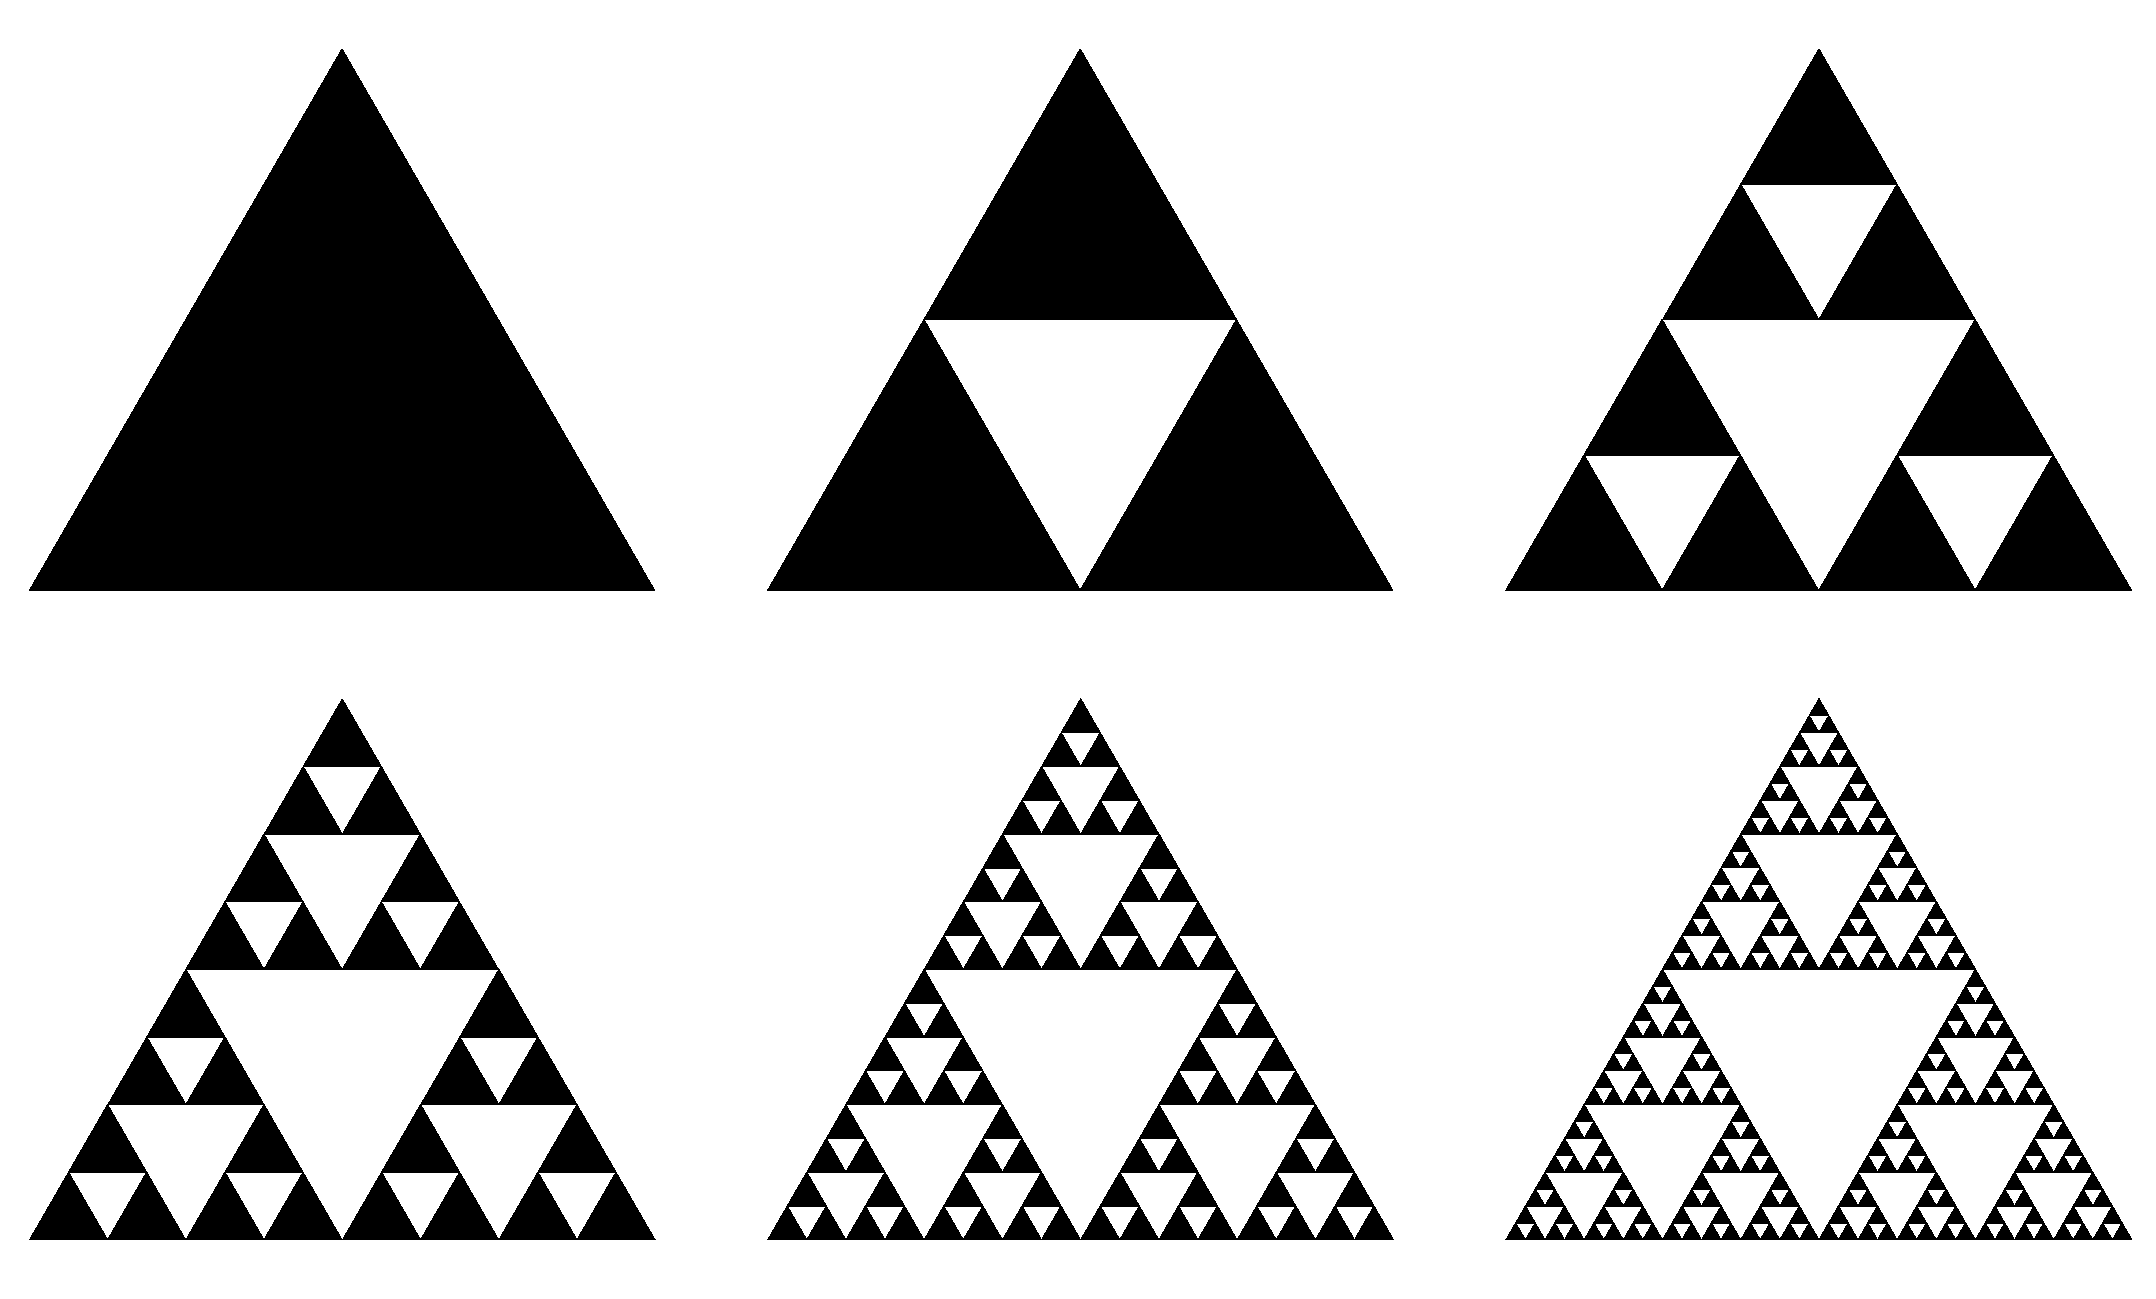
\includegraphics[width=(\imgWidth/2)]{images/sierpinski_triangle.pdf}
    \caption{Konstruktion eines Sierpinski-Dreiecks.}
    \label{fig:sierpinski_triangle}
\end{figure}

Formal kann die Erzeugung eines solchen Fraktals mithilfe eines Lindenmayer-Systems (kurz: L-System) beschrieben werden.
Dieses wurde bereits 1968 von dem Botaniker Aristid Lindenmayer vorgestellt \cite{38_lindenmayer}, wurde zunächst allerdings
nur zum Beschreiben von Wachstumsmustern in Pflanzen benutzt und erst später auf das Erstellen von geometrischen Strukturen
angepasst. \cite{39_lindenmayer_prusinkiewicz}

Ein L-System ist definiert durch das Tripel \(L = (V,\omega,P)\), wobei \(V\) eine Menge an Symbolen, \(\omega\) das
sogennante Startwort, und \(P\) eine Menge an Produktionsregeln ist. Die Menge an Symbolen \(V\), oder auch das
\textit{Alphabet}, besteht aus Variablen (Symbole, die ersetzt werden können) und Konstanten (Symbole, die nicht
ersetzt werden können). \(\omega\) ist eine nicht leere Zeichenkette bestehend aus Symbolen \(\alpha \in V\), welche den
Ursprungszustand des L-Systems darstellt. Die Produktionsregeln in \(P\) stellen alle möglichen Ersetzungsoperationen
dar und beschreiben, womit die verschiedenen Variablen ersetzt werden können. Eine solche Produktionsregel besteht
aus zwei Zeichenketten: dem Vorgänger \(\alpha\) und dem Nachfolger \(\beta\). Beim Anwenden dieser Produktion werden dann
alle Symbole in der Vorgänger-Zeichenkette mit den Nachfolger-Symbolen ersetzt: \(\alpha \rightarrow \beta\). Um nun verschiedene
Zeichenketten aus diesem L-System ableiten zu können, wird zunächst das Startwort \(\omega\) herangezogen, auf
wessen Variablen dann iterativ die vorhandenen Produktionen angewandt werden können. In jeder Iteration werden dabei
so viele Regeln wie möglich zur gleichen Zeit angewandt, was ein L-System ganz klar von formalen Grammatiken unterscheidet.
\cite{39_lindenmayer_prusinkiewicz}

\begin{figure}[t]
    \centering
    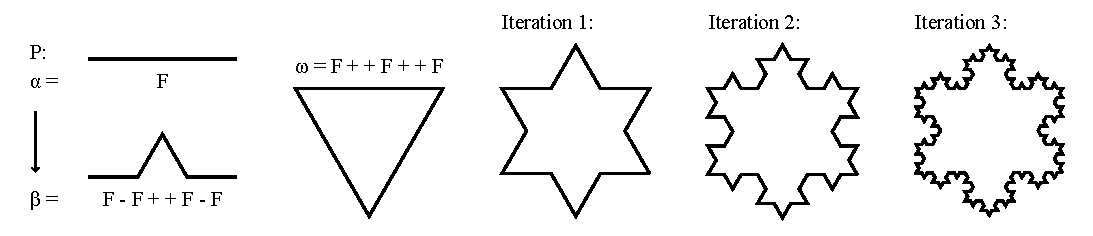
\includegraphics[width=\imgWidth]{images/koch_curve.pdf}
    \caption{Konstruktion einer Koch-Kurve durch ein L-System.}
    \label{fig:koch_curve}
\end{figure}

Aus den erzeugten Zeichenketten eines L-Systems können nun fraktale geometrische Strukturen erzeugt werden, indem man die
verwendeten Symbole z.B. als Kommandos einer Turtle-Grafik \cite{41_papert} interpretiert. Ein Beispiel hierfür ist die Erzeugung
einer Koch-Kurve \cite{40_koch}. Das entsprechende L-System kann definiert werden durch \(L = (V,\omega,P)\) mit
\(V = \{F,+,-\}\), \(\omega = F++F++F\), und \(P = \{F \rightarrow F-F++F-F\}\), wobei \(F\) das Zeichnen einer Linie,
\(+\) das Drehen der Schildkröte um 60° nach rechts, und \(-\) das Drehen der Schildkröte um 60° nach links symbolisieren.
Das entsprechende L-System und die ersten drei Iterationsschritte bei dessen Anwendung sind in Abbildung \ref{fig:koch_curve}
dargestellt. \cite{42_mcbride}

\subsection{Perlin Noise}
Aufgrund der rekursiven Struktur solcher Fraktale wird deren Berechnung schnell sehr rechenintensiv. Dies ist und war vor allem
damals für viele Anwendungsfälle ein nicht vernachlässigbares Problem. \cite{24_blatz_korn} Daher war eine nicht rekursive
Alternative nötig, welche schließlich etwas später in Form von Rauschfunktionen bzw. \textit{Noise} geliefert wurde. Der wohl
bekannteste Vertreter dieses Konzepts ist das 1985 von Ken Perlin entwickelte \cite{16_perlin} und 2002 verbesserte \cite{18_perlin}
\textit{Perlin Noise}, welches seit dessen Veröffentlichung nicht mehr aus der Welt der Computergrafik wegzudenken ist. Mithilfe von
Perlin Noise können eine Reihe von Zufallswerten erzeugt werden. Hierbei sind sich nah beieinander liegende Werte stets sehr ähnlich und
es gibt keine starken Ausschläge, weshalb der entstehende Verlauf sehr organisch wirkt. Aufgrund von dieser Eigenschaft eignet sich
Perlin Noise ebenfalls perfekt zum Erzeugen von natürlichen Strukturen. Generell ist der erzeugte Kurvenverlauf vielseitig einsetzbar
und findet somit in vielen verschiedenen Anwendungen einen Nutzen, darunter bei der Synthese von Texturen oder auch im Bereich der
Animation. \cite{17_lagae_et_al}

Neben der vielseitigen Einsetzbarkeit von Perlin Noise gibt es außerdem den Vorteil, dass dieses Verfahren sehr günstig sowohl in Bezug auf
die Berechnungszeit als auch in Bezug auf die Speicherverwendung ist. Einzelne Punkte im Verlauf lassen sich unabhängig voneinander berechnen,
wodurch sich der Berechnungsprozess wunderbar parallelisieren lässt. Dies wird mit der immer weiter voranschreitenden Entwicklung von
Grafikkarten und Prozessoren auch zu einem immer größeren Vorteil. \cite{17_lagae_et_al}

\begin{figure}[t]
    \centering
    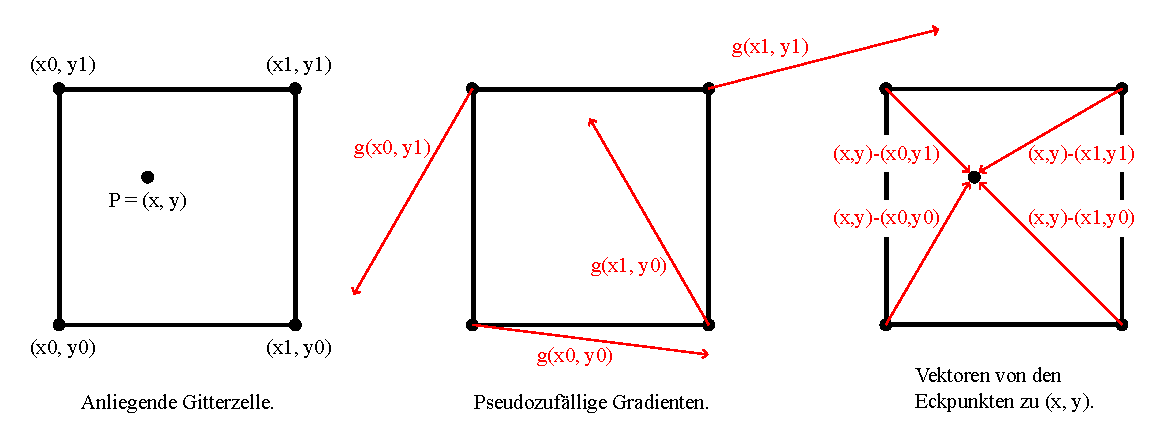
\includegraphics[width=\imgWidth]{images/perlin_noise.pdf}
    \caption{Perlin Noise: Gitterzelle und generierte Vektoren (in Anlehnung an \cite{43_zucker}).}
    \label{fig:perlin_noise}
\end{figure}

Perlin Noise kann für eine beliebige Anzahl an Dimensionen berechnet werden. Dazu wird der n-dimensionale Raum in eine reguläre gitterartige
Struktur aufgespalten. Die Punkte auf dem Gitter sind dabei all jene, die an ausschließlich ganzzahligen Koordinaten liegen. Im zweidimensionalen
Raum wäre dies also die Menge an Punkten \(\{(x, y) \ \| \ x, y \in \mathbb{N}\}\). Alle anderen Punkte im Raum befinden sich dann jeweils innerhalb
einer der von den Gitterpunkten aufgespannten Zellen. Jeder der Gitterpunkte bekommt außerdem einen pseudozufälligen Gradienten (Richtungsvektor
der Länge 1) zugeordnet. Soll jetzt der Noise-Wert für einen Punkt \(P = (x, y)\) im Raum berechnet werden, werden zunächst die Eckpunkte der
betroffenen Gitterzelle und deren zugeordnete Gradienten ermittelt. Außerdem werden die Vektoren berechnet, die von den Eckpunkten der Gitterzelle
in Richtung des gewählten Punktes zeigen. Ein solche Zelle mitsamt der dazugehörigen Vektoren ist in Abbildung \ref{fig:perlin_noise} dargestellt.
Liegen all diese Werte vor, so kann der Noise-Wert berechnet werden, indem wir den Einfluss der pseudozufälligen Gradienten auf den ausgewählten
Punkt berechnen und anschließend den gewichteten Mittelwert all dieser Einflüsse ermitteln. Der Einfluss eines einzelnen Gradienten \(g\) kann
dabei berechnet werden, indem wir das Skalarprodukt zwischen \(g\) und dem Vektor, der vom entsprechenden Eckpunkt zu \(P\) zeigt, berechnen.
Für den Gradienten \(g(x0,y0)\) würde dies wie folgt aussehen: \(g(x_0,y_0) \cdot ((x,y)-(x_0,y_0))\). Ist dies für jeden der Eckpunkte erfolgt,
so wird nun der gewichtete Mittelwert daraus berechnet. Dabei erhalten die Eckpunkte, die dem Punkt \(P\) näher sind, eine stärkere Gewichtung.
Dieser Mittelwert ist der gesuchte Noise-Wert für den Punkt \(P\). \cite{43_zucker}

\section{Inverse Verfahren}
Die bisher vorgestellten Verfahren haben alle eine Gemeinsamkeit: sie erzeugen neue Strukturen aus bereits vordefinierten Regeln. Im Anschluss
wollen wir einige Verfahren vorstellen, die etwas anders vorgehen und solche Regeln selbst erzeugen. Dabei wird beispiel-basiert gearbeitet,
d.h. die entsprechenden Verfahren erhalten eine vorgefertigte Beispielstruktur als Input. Diese werden anschließend auf bestimmte Eigenschaften und
Muster untersucht, um dann per Reverse Engineering einige Regeln ableiten zu können, mithilfe welcher neue Strukturen mit ähnlichen Eigenschaften
automatisch erzeugt werden können. Aufgrund des umgekehrten Vorgehens hierbei bezeichnen wir solche Verfahren als \textit{invers}.

\subsection{Model Synthesis und Wave Function Collapse}
Ein recht bekanntes und von vielen Spieleentwicklern genutztes Verfahren trägt den Namen \textit{\gls{ac:wfc}}. Dieses ist ein 2016 von
Maxim Gumin entwickelter Algorithmus, welcher eine Bitmap als Input entgegen nehmen kann und aus dieser Variationen ableiten kann. Hier wird also
mit gitterartigen Strukturen gearbeitet, weshalb sich \glossary{ac:wfc} perfekt zum Generieren von Pixel Art Texturen oder dem Erstellen von
Leveln in Kachel-basierten Videospielen eignet. \cite{45_gumin} Das Konzept hinter der Funktionsweise von \gls{ac:wfc} stammt allerdings
nicht von Gumin selbst, sondern beruht auf einem von Paul Merrell in 2007 vorgestelltem Verfahren namens \textit{Model Synthesis} \cite{20_merrell}.
Ein detaillierter Vergleich beider Verfahren wurde durch Paul Merrell selbst in 2021 vorgenommen \cite{46_merrell} und soll hier nicht von weiterer
Bedeutung sein. Was für uns jedoch wichtig ist, ist, dass Model Synthesis spezifisch auf das Erstellen von Modellen im dreidimensionalen Raum
abzielt \cite{20_merrell}, während \gls{ac:wfc} in seiner ursprünglichen Form ausschließlich für zweidimensionale Strukturen genutzt werden
konnte \cite{45_gumin}\cite{46_merrell}. Da diese Arbeit ebenfalls nur auf das Generieren von Strukturen im 2D abzielt, betrachten wir im Folgenden
also den \gls{ac:wfc}-Algorithmus etwas näher.

Grundlegend arbeitet \gls{ac:wfc} Gitter-basiert und mit einer Sammlung von Kacheln. Jede Kachel repräsentiert ein mögliches Muster oder eine mögliche
Form, die in eine Zelle des Gitters platziert werden kann. Nutzt man den Algorithmus z.B. zum Erstellen von Texturen, so handelt es sich dabei um eine
simple Farbe des entsprechenden Pixels. Nutzt man ihn zum Erstellen eines Levels in einem Kachel-basierten Videospiel, so kann es sich dabei auch um
detaillierte Texturen für z.B. Wasserflächen oder Wälder handeln. Um zu bestimmen, welche Kacheln letztendlich in die Zellen platziert werden können,
werden Constraints genutzt. Bevor eine neue Struktur generiert wird, werden für jede verschiedene Kachel Constraints abgeleitet, die beschreiben, neben
welchen anderen Kacheln sich diese befinden darf. \cite{45_gumin}

Nun zum Ablauf des eigentlichen Verfahrens: \gls{ac:wfc} beginnt mit einem leeren Gitter, welches ausgefüllt werden soll. Zu Beginn sind alle Positionen
in diesem Gitter vollständig unbestimmt, d.h. in jede Zelle darf jede Kachel eingetragen werden. Anschließend werden die Zellen Schritt für Schritt mit
Kacheln gefüllt. Dazu wird in jedem Schritt ein Entropie-Wert für jede Zelle berechnet, welcher beschreibt, wie viele verschiedene Kacheln dort noch
platziert werden dürfen. Es wird also geschaut, welche Kacheln sich bereits in der Nachbarschaft der ausgewählten Zelle befinden, woraufhin einige der
verfügbaren Kacheln für diese Position ausgeschlossen werden können. Im Anschluss wird die Zelle mit der niedrigsten Entropie betrachtet und für diese
zufällig eine der verfügbaren Kacheln ausgewählt und dort platziert. Dieser Vorgang wird als ``Kollabieren'' der Zelle bezeichnet (daher das ``Collapse''
im Namen des Algorithmus) und führt zu einer Anpassung der Entropie-Werte der umliegenden Zellen. Dieser Vorgang wird nun immer weiter wiederholt, bis
schließlich alle Zellen nach diesem Prinzip kollabiert werden konnten oder es an irgendeiner Stelle zu einem Widerspruch kommt. Ein Widerspruch liegt
vor, wenn für eine der noch offene Zellen ein Entropie-Wert von \(0\) berechnet wird und es somit keine Kacheln mehr gibt, die dort platziert werden
können. Tritt dies auf, so muss der gesamte Vorgang wiederholt werden. Maxim Gumin zufolge tritt dieses Problem in der Praxis allerdings ``überraschend
selten'' auf. \cite{45_gumin} Einige Beispiele für Strukturen, die nach diesem Vorgehen generiert werden können, lassen sich in Abbildung \ref{fig:wfc}
finden. Das dritte Beispiel hier könnte z.B. als Layout für einen Dungeon verwendet werden.

\begin{figure}[t]
    \centering
    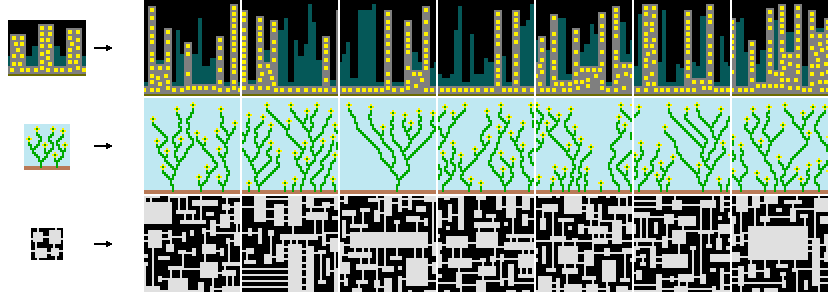
\includegraphics[width=\imgWidth]{images/wfc.png}
    \caption{Wave Function Collapse: Beispielstrukturen und generierte Variationen \cite{45_gumin}.}
    \label{fig:wfc}
\end{figure}

\subsection{Nutzen von partieller Symmetrie}
% wfc kann mit wenig aufwand recht beeindruckende Ergebnisse erzeugen, ist jedoch in seiner Anwendung sehr limitiert (nur gitter-basiert)
% daher anderer Ansatz: Bokeloh et al., Quelle 3

\subsection{Inverses Ableiten einer Graph-Grammatik}
% Merrell, Quellen 1-2
